\chapter{绪论}

\section{模式(字符串)匹配问题}

模式匹配(Pattern Matching, 简称PM), 一直以来都是计算机科学的核心问题之
一。 这里的“模式”特指字符串。 对于很多应用, 例如模式识
别 \cite{Yan2016}, \cite{Xiao2016}, 本体匹配 \cite{Xue2015}
\cite{Xue2016}, 文本分类 \cite{Tang2015} \cite{Zhang2016}, 系统安
全 \cite{Dien2014,Malhotra2016,Fan2016},入侵检测系
统 \cite{Kim2015,Arney2016,Sadotra2016,Lee2017} 等等, 模式匹配算法都是
最为基本而重要的操作。根据待匹配模式的数量,模式匹配技术可以分为两类:
单模式匹配(SPM)和多模式匹配(MPM)。

\begin{figure}[!h]
  \centering
  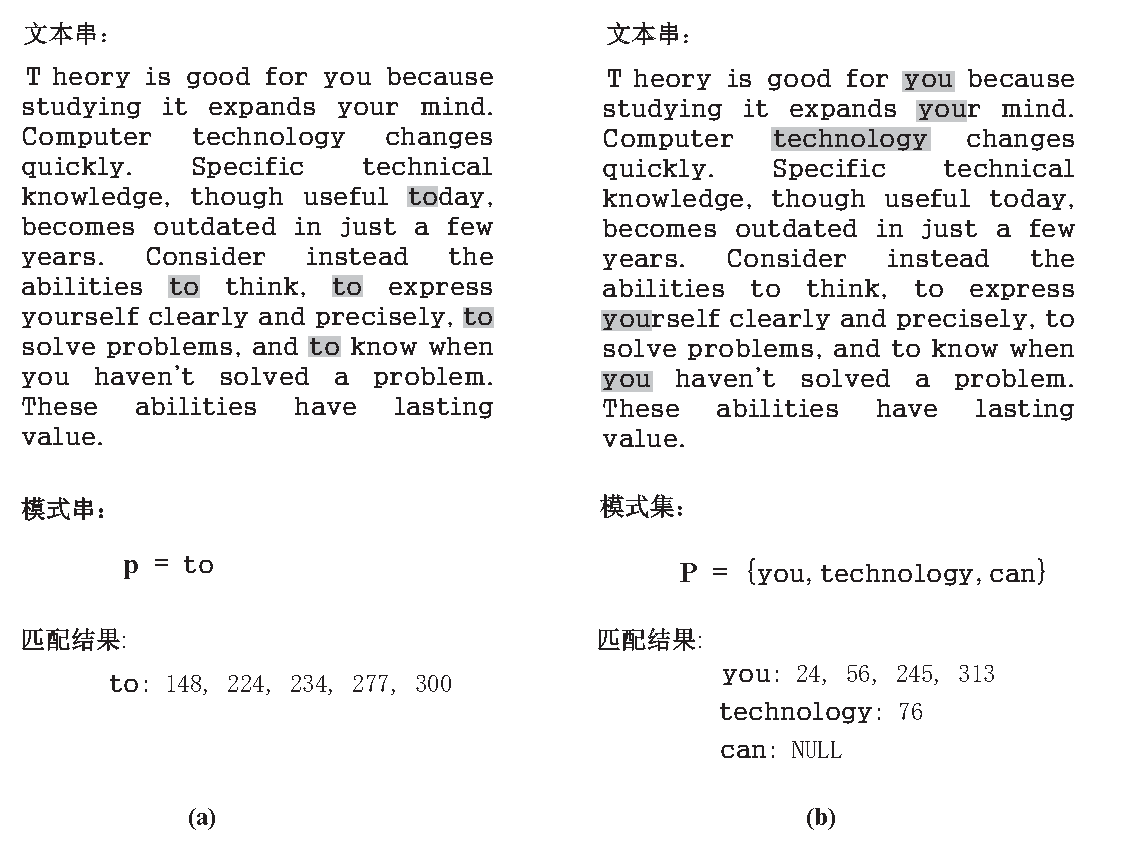
\includegraphics[height=8cm ,width=12cm]{figures/1_Introduction/SPM_MPM.eps}
  \caption{(A) 单模式匹配示例。(B) 多模式匹配示例。}
  \label{fig:SPM_MPM}
\end{figure}


\subsection{单模式匹配}

单模式匹配算法要求在文本串中寻找给定模式串的所有出现位置。如
图 \ref{fig:SPM_MPM } (A) 所示, 给定文本串与模式$to$, 经过匹配发现,模
式串$to$ 出现于文本串中的位置为: 148, 224, 234, 277, 300。

最简单的单模式匹配算法,需要对文本串中的每一个位置与模式串进行逐字符的
比较,一旦出现字符失配,将直接移动到文本串的下一个位置进行匹配。很明显,
当文本串的长度为$n$且模式串的长度为$m$时,这种简单的模式匹配算法的时间
复杂度为$O(m \cdot
n)$。当文本串形如$aaa \dots
a$及模式串为$aaab$时,将出现最坏情况。为此,有更加高效的单模式匹配算法
被提出,最著名的包括KMP \cite{Knuth1977}算法 和 BM \cite{Boyer1977} 算
法。下面将简单介绍这两种算法的核心思想。

1. \textbf{KMP(Knuth-Morris-Pratt)算法}

KMP算法的核心思想在于,一旦匹配失败,可以充分利用已经匹成功的子串信息,
让模式串向右移动尽可能多的位置。右移的距离是这样计算的:在已经匹配的模
式串子串中,找出最长的相同的前缀和后缀,然后向右移动使它们重叠。如
图\ref{fig:KMP}(A)所示,在当前匹配中,文本串中的位置10($i=10$)和模式串
中的位置8($j=8$)出现失配,根据已经匹配成功的子串即$abcdaabc$的信息:该
子串相等的最长前缀与最长后缀是$abc$, 将模式串向右移动使得这两部分相重合,
如图 \ref{fig:KMP} (B)
所示。此时,文本串中当前待匹配位置$i$不变,而模式串中当前待匹配位
置$j$变为3,分别从位置$i$和$j$开始对文本串和模式串进行逐字符比较。KMP算
法在匹配过程中,文本串中的当前匹配位置$i$永不减小,只是当匹配失败时,根
据模式串中的失配位置,来调整模式串中的下一次与文本串位置$i$相比较的位置。
因此,需要知道在失配时,下一次应当用模式串的哪个位置与文本串进行比较。
为此对模式串进行预处理,为其建立失配数组$Next$(如图 \ref{fig:KMP} (C)所
示),
如果当前在模式串的位置$j$失配时,下一次将用模式串的位置$Next[j]$来与文
本串进行比较,预处理过程的时间复杂度为$O(m)$($m$为模式串长度)。 由于匹
配过程中, 文本串中的位置$i$永不回溯,所以KMP算法的时间复杂度为$O(m+n)$
($n$为文本串长度)。

\begin{figure}[!h]
  \centering
  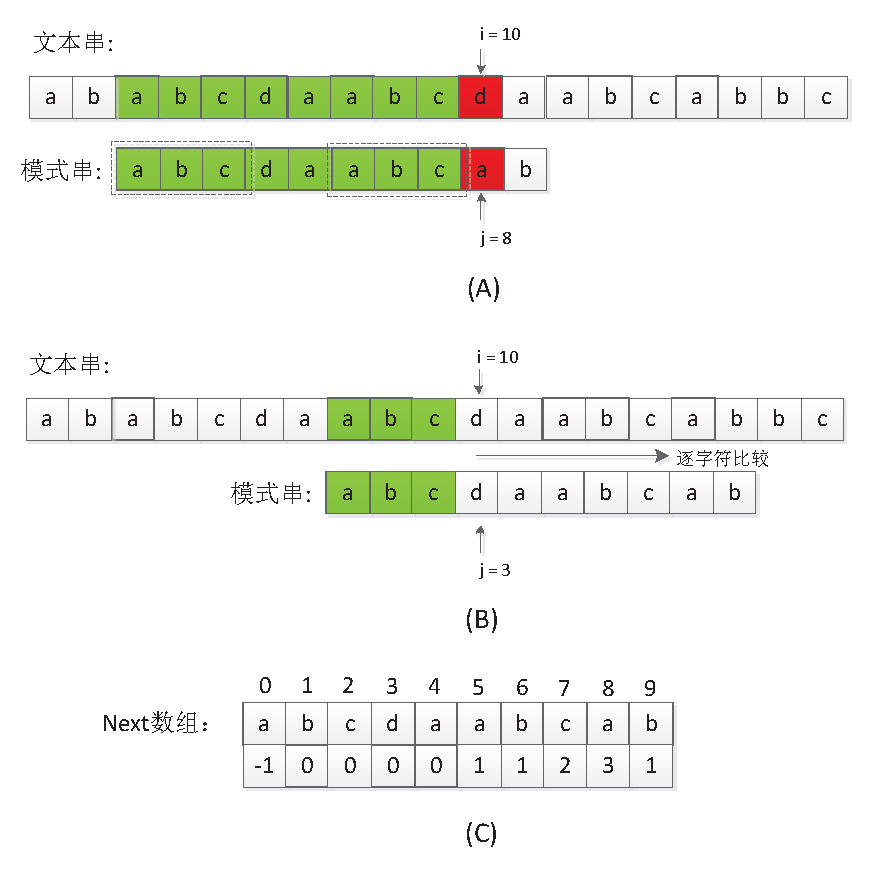
\includegraphics[height=10cm ,width=12cm]{figures/1_Introduction/KMP.eps}
  \caption{KMP算法示例。(A) 第一轮匹配。(B) 第二轮匹配。(C) 模式串
    的Next数组。}
  \label{fig:KMP}
\end{figure}


2. \textbf{BM(Boyer-Moore)算法}

尽管KMP算法具有线性的时间复杂度,可其实际的速度却并不快。在实际应用当中
(比如各类字处理软件中的字符串查找功能),最常用的单模式匹配算法是BM算
法 \cite{Boyer1977}, 及其诸多变体。BM算法最高效之处在于通过使用“坏字
符”规则,其可以快速跳过文本串中大量的不可能出现匹配的位置。如
图 \ref{fig:BM} (A) 所示,BM算法采用从右到左的方向对模式串与文本串进行
比较,由于第一次比较即失配且文本串中相应的字符$s$没有出现在模式串中,因
此可以将模式串整体向右移动到$s$的下一个字符处,然后再别从位
置13($i=13$)和位置6($j=6$),从右向左地对文本串和模式串进行比较,如
图 \ref{fig:BM} (B)
所示。由于再次失配,且文本串中的字符$p$出现于模式串中,因此将模式串向右
移动2个位置,使两个串中的$p$字符对齐,如图\ref{fig:BM}(C)所示。由于BM算
法在每次匹配失败时,都将根据文本串中的失配字符来移动模式串,因此需要对
整个字符集进行预处理构建坏字符表(表长为$|\Sigma|$,即字符集大小),当
匹配失败时用文本串中的失配字符作为索引来查找坏字符表,来决定需要将模式
串向后移动多少位。BM算法最坏情况的时间复杂度为$O(n \cdot m)$,但是在实
际中很少出现这样的情况。

\begin{figure}[!h]
  \centering
  \includegraphics[height=10cm ,width=12cm]{figures/1_Introduction/BM.eps}
  \caption{BM算法示例。(A) 第一轮匹配。(B) 第二轮匹配。(C) 第三轮匹配。}
  \label{fig:KMP}
\end{figure}

\subsection{多模式匹配}

多模式匹配要求找出给定模式集中每一个模式串在文本串中的所有出现位置。如
图 \ref{fig:SPM_MPM} (B) 所示,给定模式集
$P={can, you, technology}$及文本串,通过多模式匹配发现, 模式串$you$出现
了4次, 模式串$technology$出现了1次, 模式串$can$在文本串中没有出现。

目前,多模式匹配算法的主要流程是先对模式集进行预处理,构建合适的数据结
构来存储和组织模式集中的模式串,然后用构建好的数据结构和文本进行比较,
一次性找出所有模式集的出现位置。 比较著名的多模式匹配算法包括 AC
\cite{Aho1975} 和 WM \cite{Wu1994} 算法。

1. \textbf{AC(Aho-Corasick)算法}

AC算法是经典的多模式匹配算法,它是KMP算法在多模式环境下的推广,具有线性
时间复杂度。目前,各种AC算法的变体在实际当中被广泛应用。AC算法通过为模
式集构造一个有限状态自动机(DFA),然后将文本串中的每一个字符输入到自动机
中进行状态转移,来实现多模式匹配。图 \ref{fig:AC} 所示的是为模式
集$P={he, his, she, hers}$ 所构造的AC自动机,图中实线箭头及对应字符表示,
在当前状态遇到该字符时应该跳转到的状态,虚线表示在当前状态无匹配字符时,
应该跳转到的状态,图中绿色的状态,表示匹配成功状态。 匹配时,AC算法将从
状态0开始,连续不断地读入文本串中的字符,并根据所读入的字符进行状态跳转,
一旦到达匹配成功状态,将输出匹配到的模式串。 举例说明,假设文本串
为$hers$, 初始状态为0, 第一个文本串字符为$h$, 则自动机将跳转到状态1;下
一个输入字符为$e$,
将跳转到状态2,同时成功匹配模式串$he$并将其输出;下一个字符为$r$,将跳
转到状态8;最后一个字符为$s$,跳转到状态9,并输入匹配成功的模式
串$hers$。传统的AC算法对字符集大小非常敏感,对于较大的字符集,算法所构
造的自动机将会消耗大量的空间,且在实际应用中性能较低。


\begin{figure}[!h]
  \centering
  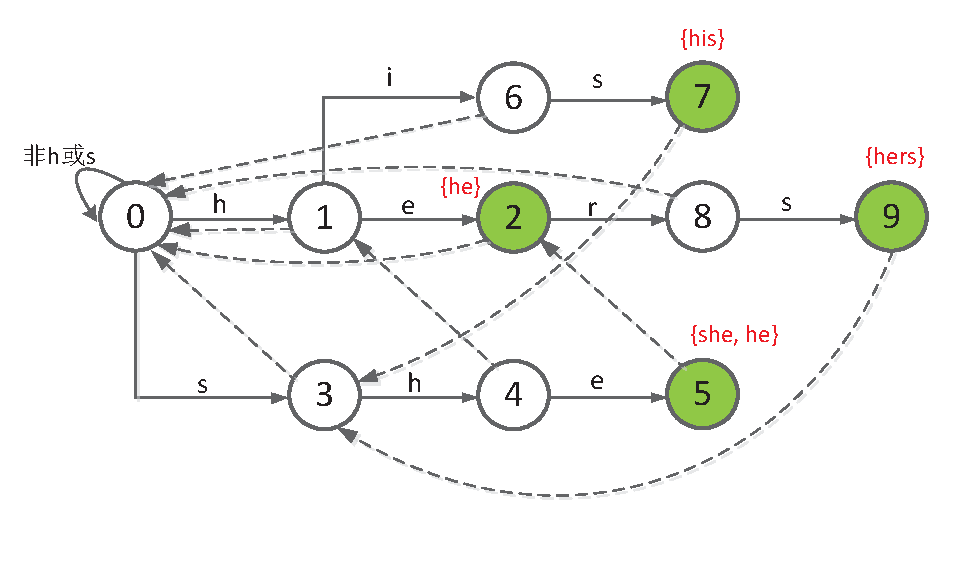
\includegraphics[height=9cm ,width=13cm]{figures/1_Introduction/AC.eps}
  \caption{为模式集$P=\{he, his, she, hers\}$所构建的AC自动机。}
  \label{fig:AC}
\end{figure}

2. \textbf{WM(Wu-Manber)算法
}

WM算法是BM算法在多模式环境下的推广,BM算法采用“坏字符”规则在文本中进
行跳跃,而WM算法采用“坏字符块”块进行跳跃,增加了跳跃的可能性。算法会
为模式集构建3个表结构:哈希表,跳转表和前缀表。然后,在文本中使用一个长
为lsp(即最短模式串长)的匹配窗口,选择待匹配的文本。
